\def\resdir{3protocoles}

% ----------------------------------------------------------------------
\section{Protocoles}
% ----------------------------------------------------------------------


% ----------------------------------------------------------------------
\begin{frame}

\centering
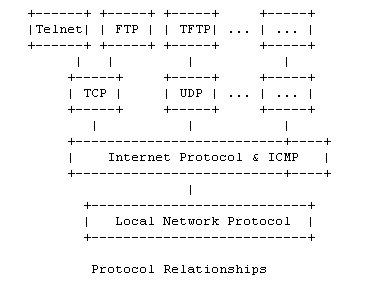
\includegraphics[width=\textwidth]{\resdir/protocol_relationship.jpg}

\end{frame}
% ----------------------------------------------------------------------




% ----------------------------------------------------------------------
\subsection{Local Network Protocol}
% ----------------------------------------------------------------------

% ----------------------------------------------------------------------
\begin{frame}{Local Network Protocol}

	\begin{block}<+-> {R�seaux avant Internet}
	\begin{itemize}
		\item Local = Non-�tendu
		\item \`A l'origine : \textit{ALOHAnet}
		\item Un seul m�dia de communication
		\item Protocole principal : \textit{Ethernet}
	\end{itemize}					
	\end{block}
		
\end{frame}
% ----------------------------------------------------------------------

% ----------------------------------------------------------------------
\begin{frame}

	\centering
	
	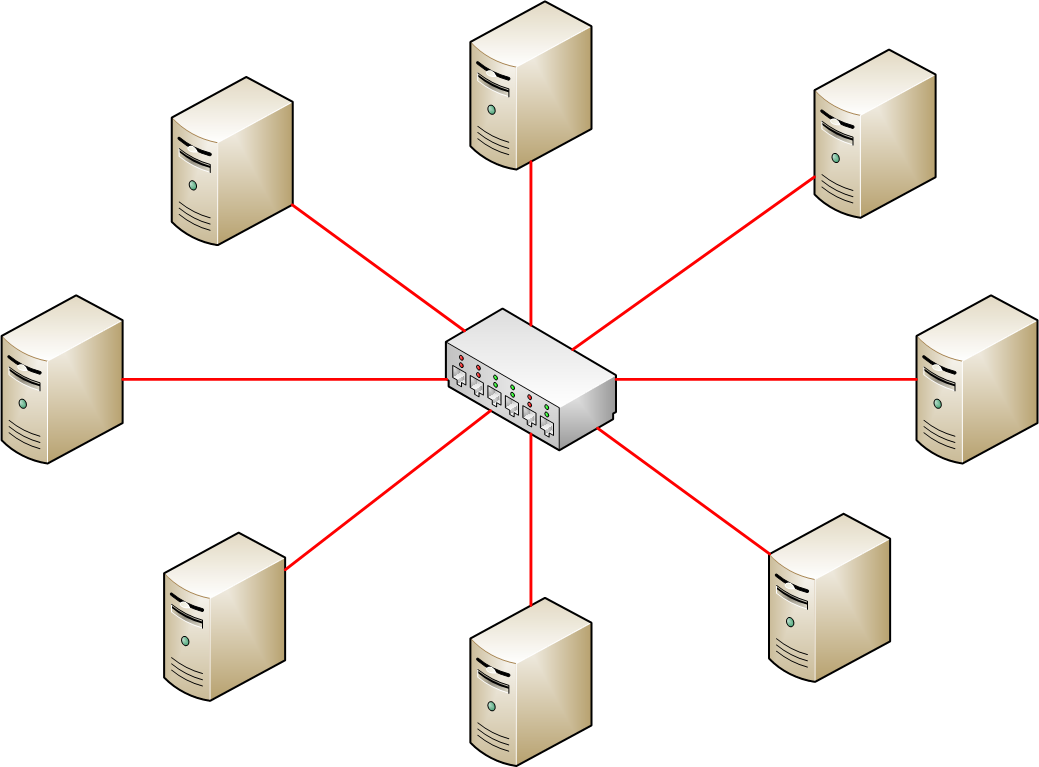
\includegraphics[height=0.6\textheight]{\resdir/ethernet}
	
	\begin{block}<+-> {Topologie}
		\begin{itemize}
			\item En \'Etoile
			\item Autour d'un hub ou d'un switch
		\end{itemize}
	\end{block}
	
\end{frame}
% ----------------------------------------------------------------------

% ----------------------------------------------------------------------
\begin{frame}
	\begin{columns}
	
	\column{0.5\textwidth}
		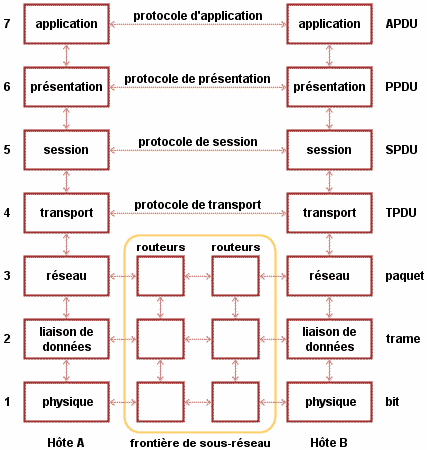
\includegraphics[height=0.8\textheight]{\resdir/osi}
	
	\column{0.5\textwidth}
		\begin{block}<+-> {Ethernet}
			\begin{itemize}
			\item Protocole R�seau local
			\item Unique ligne de communication
				\item Impl�mentation des couches
				\begin{itemize}
					\item Liaison
					\item Physique
				\end{itemize}
				\item Ether - Net(work)
				\item Bas� sur l'adresse MAC
				\begin{itemize}
					\item Media Access Control 
				\end{itemize}
				\item \'Echange de \textit{Trames}
				\item 10 Mb/s � 10 Gb/s
			\end{itemize}
		\end{block}
		
	\end{columns}		
\end{frame}
% ----------------------------------------------------------------------






% ----------------------------------------------------------------------
\subsection{Internet}
% ----------------------------------------------------------------------


% ----------------------------------------------------------------------
\begin{frame}{Inter-Network Protocols}

	\begin{block}<+-> {Deux niveaux g�n�riques basiques}
	\begin{itemize}
		\item R�seau Local : Ethernet
		\item R�seau Global : Internet
			\begin{itemize}
			\item IP : Internet Protocol
			\item ICMP : Internet Control Message Protocol
			\item GGP : Gateway to Gateway Protocol
			\end{itemize}
		\end{itemize}					
		\end{block}
		
		\centering
		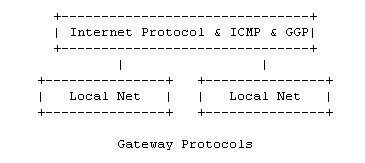
\includegraphics[width=\textwidth]{\resdir/gateways_protocol.jpg}

\end{frame}
% ----------------------------------------------------------------------

% ----------------------------------------------------------------------
\begin{frame}{Internet}

	\centering
	
	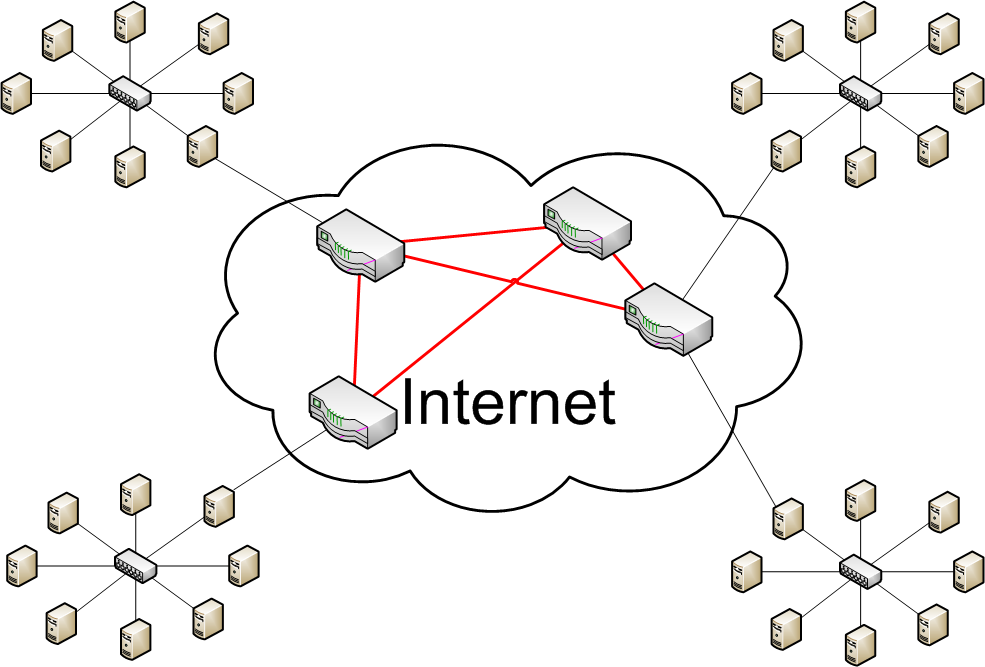
\includegraphics[height=0.6\textheight]{\resdir/internet}
	
	\begin{block}<+-> {Topologie}
		\begin{itemize}
			\item Quelconque
			\item R�seaux locaux en ``bordure''
			\item Inter-Net(work)
		\end{itemize}
	\end{block}
	
\end{frame}
% ----------------------------------------------------------------------


% ----------------------------------------------------------------------
\begin{frame}
	\begin{columns}
	
	\column{0.5\textwidth}
		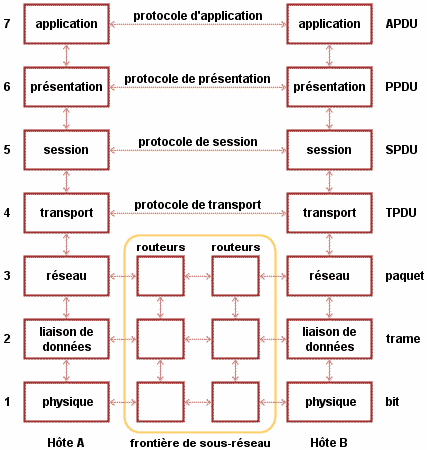
\includegraphics[height=0.8\textheight]{\resdir/osi}
	
	\column{0.5\textwidth}
		\begin{block}<+-> {IP : Internet Protocol}
			\begin{itemize}
			\item Protocole R�seau de R�seaux
			\item D�crit dans la RFC 791							
			\item Rout�
			\item Impl�mentation de la couche
				\begin{itemize}
					\item R�seau
				\end{itemize}
				\item Bas� sur l'adresse IP
				\begin{itemize}
					\item IPv4 ou IPv6
				\end{itemize}
				\item \'Echange de \textit{Paquets}
				\item Ne g�re pas les erreurs
			\end{itemize}
		\end{block}
		
	\end{columns}		
\end{frame}
% ----------------------------------------------------------------------

% ----------------------------------------------------------------------
\begin{frame}

	\centering
	
	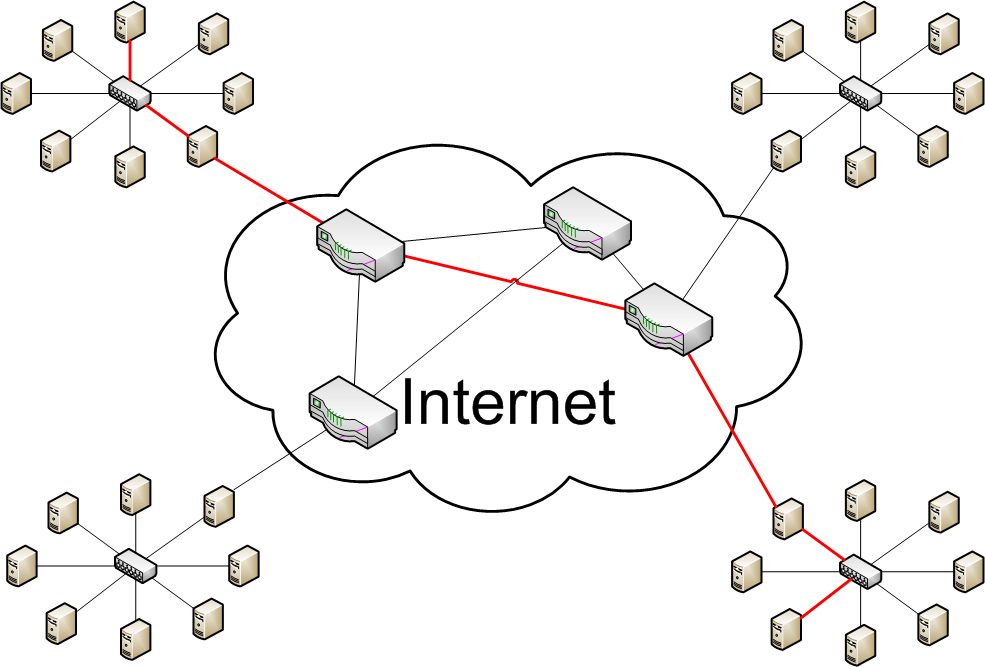
\includegraphics[height=0.6\textheight]{\resdir/bout-en-bout}
	
	\begin{block}<+-> {Communications de Bout-en-Bout}
		\begin{itemize}
			\item Entre deux machines terminales
		\end{itemize}
	\end{block}
	
\end{frame}
% ----------------------------------------------------------------------



% ----------------------------------------------------------------------
\begin{frame}
	\begin{columns}
	
	\column{0.5\textwidth}
		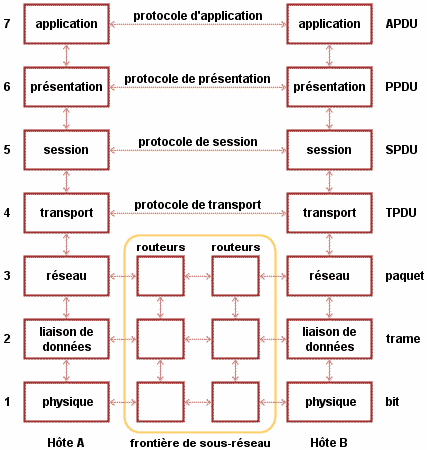
\includegraphics[height=0.8\textheight]{\resdir/osi}
	
	\column{0.5\textwidth}
		\begin{block}<+-> {ICMP : Internet Control Message Protocol}
			\begin{itemize}
			\item Protocole R�seau de R�seaux
			\item D�crit dans la RFC 792							
			\item Rout�
			\item Agit au niveau de la couche
				\begin{itemize}
				\item R�seau
				\end{itemize}
			\item G�re les erreurs et l'administration
				\begin{itemize}
				\item P.ex. msg (echo) pour ping
				\end{itemize}
			\end{itemize}
		\end{block}
		
	\end{columns}		
\end{frame}
% ----------------------------------------------------------------------

% ----------------------------------------------------------------------
\begin{frame}
	\begin{columns}
	
	\column{0.5\textwidth}
		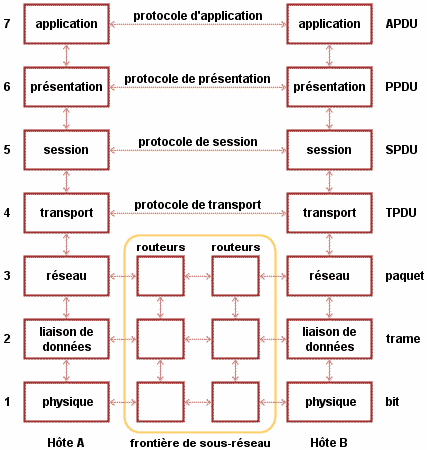
\includegraphics[height=0.8\textheight]{\resdir/osi}
	
	\column{0.5\textwidth}
		\begin{block}<+-> {GGP : Gateway to Gateway Protocol}
			\begin{itemize}
			\item Obsol�te : BGP Border Gateway Protocol
			\item D�crit dans la RFC 4271		
			\item Agit au niveau de la couche
				\begin{itemize}
				\item R�seau
				\end{itemize}
			\item MAJ des routes entre routeurs
				\begin{itemize}
				\item Entre Autonomous Systems (AS)
				\end{itemize}
			\end{itemize}
		\end{block}

	\end{columns}
\end{frame}
% ----------------------------------------------------------------------




% ----------------------------------------------------------------------
\subsection{Protocoles de Communication Applicatives}
% ----------------------------------------------------------------------



% ----------------------------------------------------------------------
\begin{frame}{Protocoles de Communication Applicatives}

\centering
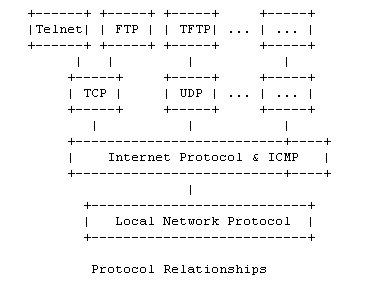
\includegraphics[width=0.8\textwidth]{\resdir/protocol_relationship.jpg}

\end{frame}
% ----------------------------------------------------------------------


% ----------------------------------------------------------------------
\begin{frame}{Protocoles de Communication Applicatives G�n�riques}

	\centering
	
	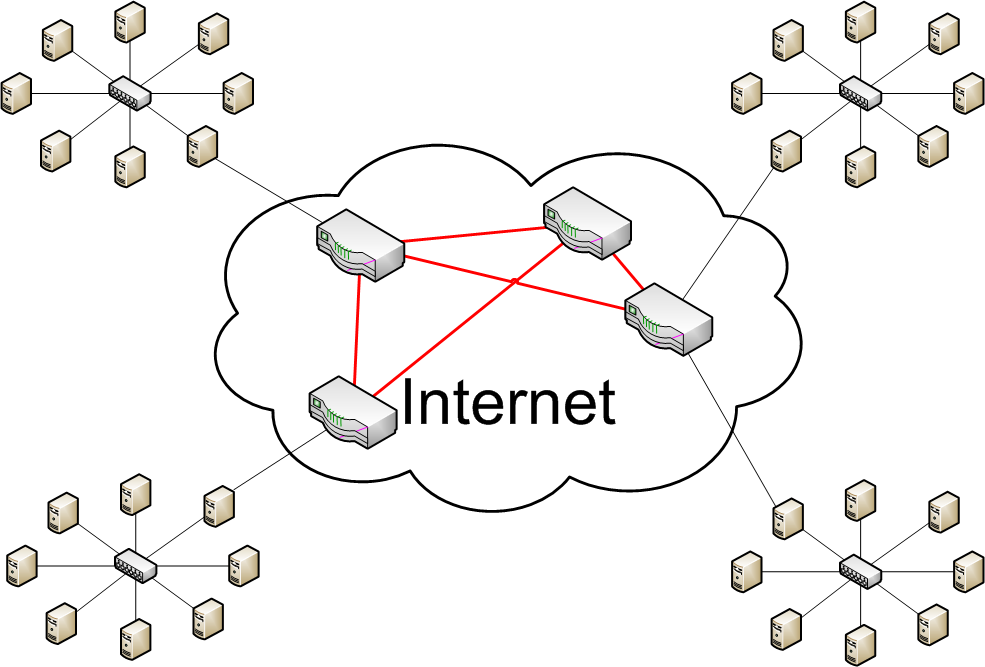
\includegraphics[height=0.4\textheight]{\resdir/internet}
	
	\begin{block}<+-> {Communications de Bout-en-Bout}
		\begin{itemize}
			\item Entre deux applications
			\item Gr�ce � la notion de \textit{port}
			\item Deux protocoles principaux
				\begin{itemize}
				\item TCP : Transmission Control Protocol (connect�)
				\item UDP : User Datagram Protocol  (d�connect�)
				\end{itemize}
		\end{itemize}
	\end{block}
	
\end{frame}
% ----------------------------------------------------------------------

% ----------------------------------------------------------------------
\begin{frame}
	\begin{columns}

	\column{0.5\textwidth}
		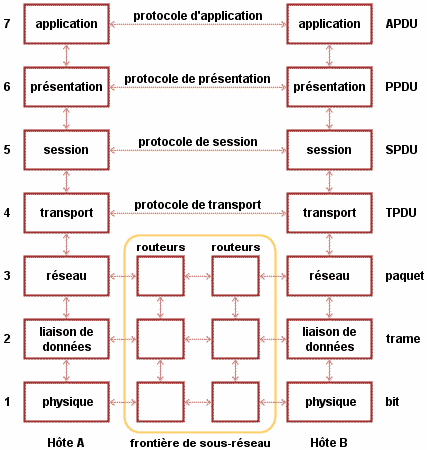
\includegraphics[height=0.8\textheight]{\resdir/osi}

	\column{0.5\textwidth}
		\begin{block}<+-> {TCP/UDP}
			\begin{itemize}
			\item Protocole Port � Port
			\item D�crits dans les RFC 793/768						
			\item Impl�mente la couche
				\begin{itemize}
				\item Transport (4)
				\item Session pur TCP (5)
				\end{itemize}
			\item Transporte l'information
				\begin{itemize}
				\item Entre deux applications
				\item Plus ou moins de services
				\end{itemize}
			\end{itemize}
		\end{block}

	\end{columns}		
\end{frame}
% ----------------------------------------------------------------------




% ----------------------------------------------------------------------
\begin{frame}{Protocoles de Communication Applicatives Sp�cifiques}

\centering
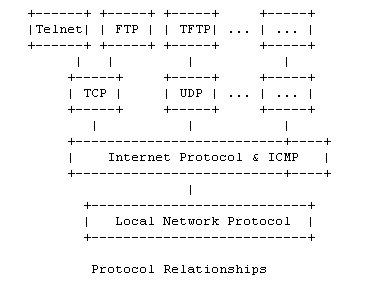
\includegraphics[width=0.8\textwidth]{\resdir/protocol_relationship.jpg}

\end{frame}
% ----------------------------------------------------------------------


% ----------------------------------------------------------------------
\begin{frame}{Protocoles de Communication Applicatives Sp�cifiques}

	\centering
	
	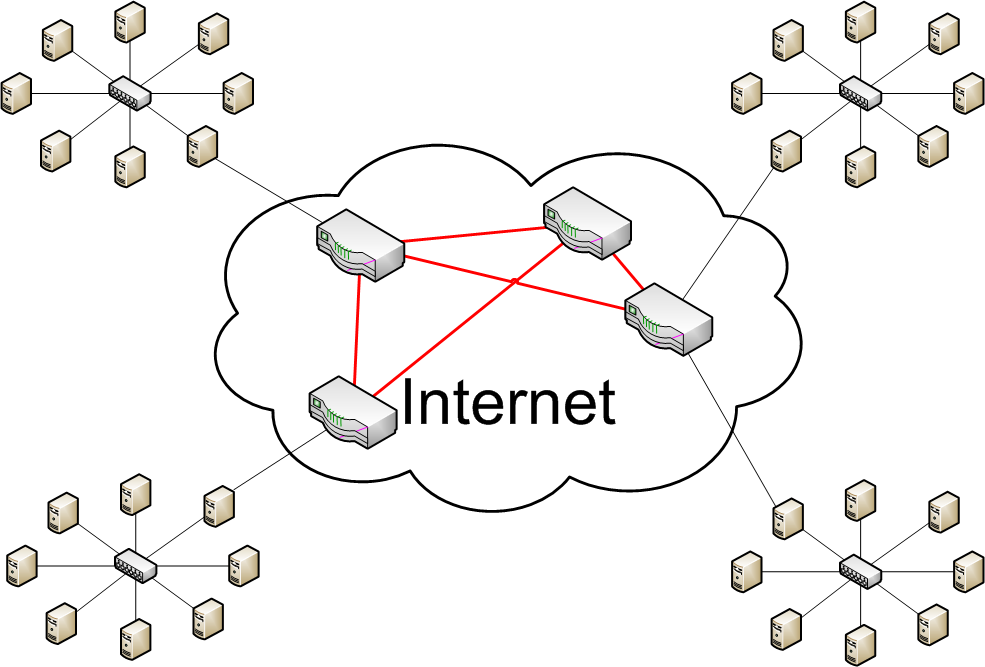
\includegraphics[height=0.4\textheight]{\resdir/internet}
	
	\begin{block}<+-> {Ajoute du service}
		\begin{itemize}
			\item D�di� � une application particuli�re
			\item Tr�s nombreux
				\begin{itemize}
				\item Telnet, FTP, Kad, AIM, Jabber
				\item Bas�s sur TCP/IP ou UDP/IP
				\end{itemize}
		\end{itemize}
	\end{block}
	
\end{frame}
% ----------------------------------------------------------------------

% ----------------------------------------------------------------------
\begin{frame}
	\begin{columns}
	
	\column{0.5\textwidth}
		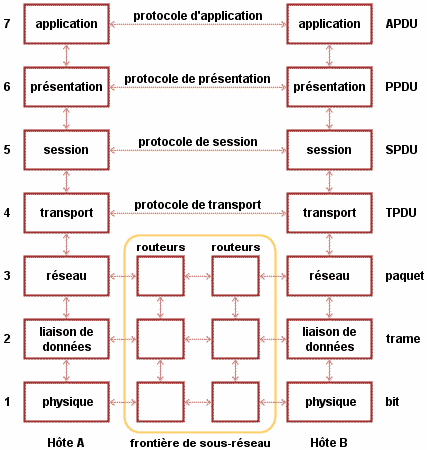
\includegraphics[height=0.8\textheight]{\resdir/osi}
	
	\column{0.5\textwidth}
		\begin{block}<+-> {Sp�cifiques}
			\begin{itemize}						
			\item Impl�mente la couche
				\begin{itemize}
				\item Application (7)
				\end{itemize}
			\item Empaquette l'information
				\begin{itemize}
				\item Dans un but pr�cis
				\end{itemize}
			\item Supporte les \textit{services}
			\end{itemize}
		\end{block}
		
	\end{columns}		
\end{frame}
% ----------------------------------------------------------------------

% ----------------------------------------------------------------------
\begin{frame}{Conclusion}
		
	\centering
	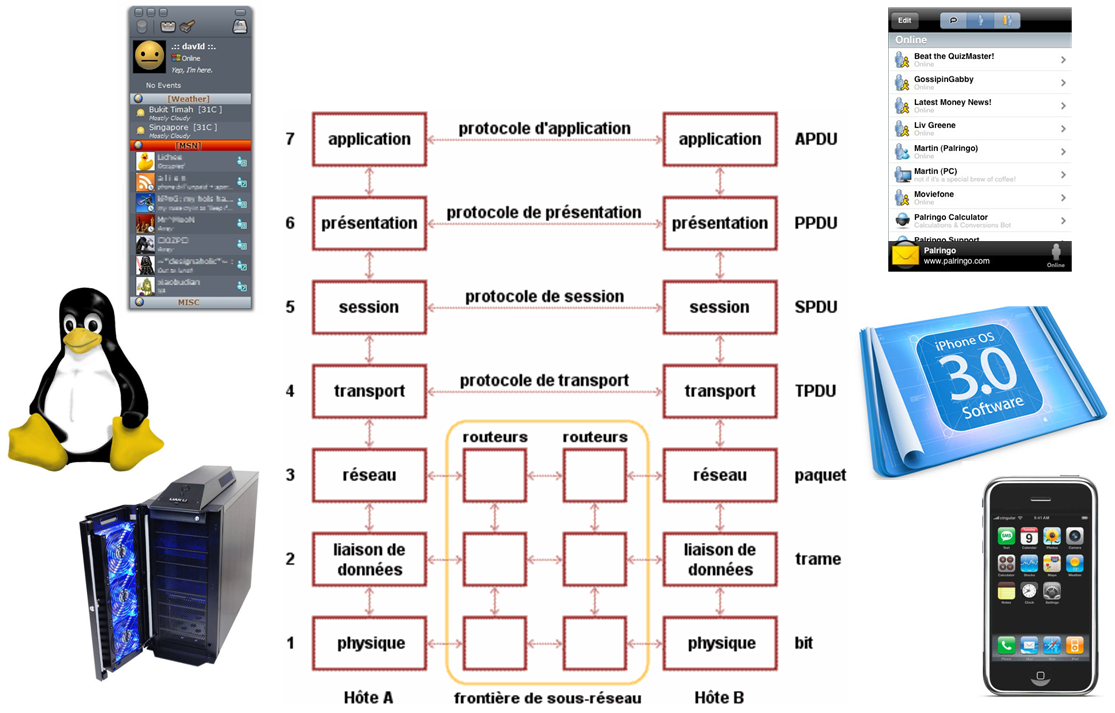
\includegraphics[height=0.8\textheight]{\resdir/osi++}

\end{frame}
% ----------------------------------------------------------------------
